\chapter{Introduction}\label{chap:introduction}
    \paragraph{}Notre projet a pour but d'élaborer un algorithme capable de trouver, dans plusieurs situations d'une partie de Go si un groupe peut survire ou non. Pour cela nous avons besoin de tout construire depuis zéro, construire la structure de base du jeu, y implémenter les règles pour finir par créer l'algorithme nécessaire à la résolution d'un problème de vie ou de mort.
    
    \section{Présentation du Jeu de Go}
        \subsection{Histoire du Go.}
            \paragraph{}Le Jeu de Go est un jeu de plateau à 2 joueurs né en Chine il y a plusieurs milliers d'années, c'est le plus ancien jeu de stratégie combinatoire abstrait connu actuellement, on raconte qu'il fut créé pendant la période chinoise des Printemps et Automnes.
            
            \paragraph{}Malgré le fait qu'il soit très ancien, le Jeu de Go continue de profiter d'une grande notoriété dans les pays Asiatiques, notamment en Chine, en Corée et au Japon où il a vu naître sa forme actuelle au XVe Siècle pour beaucoup plus récemment s'exporter en Occident où nous l'avons découvert.
            
            \paragraph{}Il a subi ces dernières années une réelle attention de la part des grands de l'informatique notamment Facebook et Google qui se sont battus pendant un longue période pour confectionner une intelligence artificielle capable de battre n'importe quel humain au Go, c'est là que Google DeepMind a réussi avec Alpha Go en 2015 et a ainsi battu le meilleur joueur de Go dans les années 2000 Lee Sedol, sauf à la quatrième parti où celui-ci à vaincu la bête.
            
            \paragraph{}C'est à l'heure actuelle le plus grand rempart jamais franchi dans le domaine du DeepLearning. Cela explique l'engouement actuel autour de l'intelligence artificielle de beaucoup d'entreprises. Réussir ce challenge est alors un tournant symbolique, celui où les ordinateurs surpassent les humains dans une activité que l'on pensait propre à l'humain.
    
        \subsection{Règles du Jeu}
            \paragraph{}Le Jeu de Go se joue à 2 joueurs, chacun d'eux pose à leur tour une pierre d'une couleur distincte sur un plateau quadrillé appelé Goban. Le but est de contrôler le plus vaste territoire, chacun se bat alors avec ses pierres pour envahir le territoire de l'autre tout en protégeant les leur  ! Il est aussi possible de capturer les groupes ennemis, nous faisant alors gagner des points que nous comptabilisons en plus des points rapportés par les territoires que nous possédons. Le gagnant est finalement celui qui obtient le plus de points.


    \section{Méthodologie de travail et environnement technique}
        \subsection{Méthodologie de gestion des versions de codes : GIT}
            \paragraph{}Ayant un module nous dispensant des cours sur cette plate-forme très pratique qu'est GIT, nous avons trouver ça intéressant d'utiliser celle-ci, et pour sûr nous ne l'avons pas regretter ! Chacun peut avancer en équipe et se passer le "témoin" à la manière d'une course de relais sauf que tout le monde peut avancer en même temps sur des points différents ! Malheureusement il y a aussi de légers désagréments, notamment lorsque tout le groupe ne code pas sur la même plate-forme. Cela engendre parfois des problèmes de compatibilité mais au final cela permet aussi une plus grande flexibilité sur le rendu final.
            
            \paragraph{}De plus, lorsque un membre fait des mauvaises modifications sans que nous nous en rendions compte,  et que un peu plus tard tandis que nous buttions sur une erreur, nous réalisons alors que l'erreur venait de là... Heureusement dans sa globalité GIT fut un fabuleux outil que nous utiliserons sans doute pour nos futurs projets. Ainsi que la diversité des système d'exploitation permet aussi d'avoir une portabilité du programme et des débugages différents.
            L'intégralité de notre projet, ses avancées, etc sont disponibles via GIT à l'adresse suivante : \href{https://github.com/Victor333Huesca/Jeu\_de\_Go}{www.github.com/Victor333Huesca/Jeu\_de\_Go}

        \subsection{Choix des technologies}
            \subsubsection{Le C++}
                \paragraph{}Le choix s'est trouvé évident, cela faisait bientôt 2 ans que nous étudions ce langage, plus pour d'autres, d'autant plus que ce soit pour la programmation objet et l'optimisation mémoire celui-ci reste l'un des meilleurs pour exceller sur ces deux plans.
        
            \subsubsection{SFML}
                \paragraph{}La SFML est une bibliothèque originellement destinée au langage C++ mais portée également vers d'autres langages divers et variés. Celle-ci permet -entre autre- un affichage graphique, des outils système, réseau et même audio.\\
                Notre choix s'est porté sur celle-ci car elle est extrêmement bien documentée (en français en plus) et elle présente un bon rapport entre simplicité d'utilisation et possibilités apportées.

        \subsection{Diagramme de tâche prévisionnel Gantt}  
            \paragraph{}Afin de ne pas s'égarer dans le c\oe ur du projet, nous nous sommes réunis pour planifier les étapes clef du projet. Nous nous somme servis de la méthode de Gantt qui est assez intuitive. 
            
            \begin{figure}[h!]
            \centering
            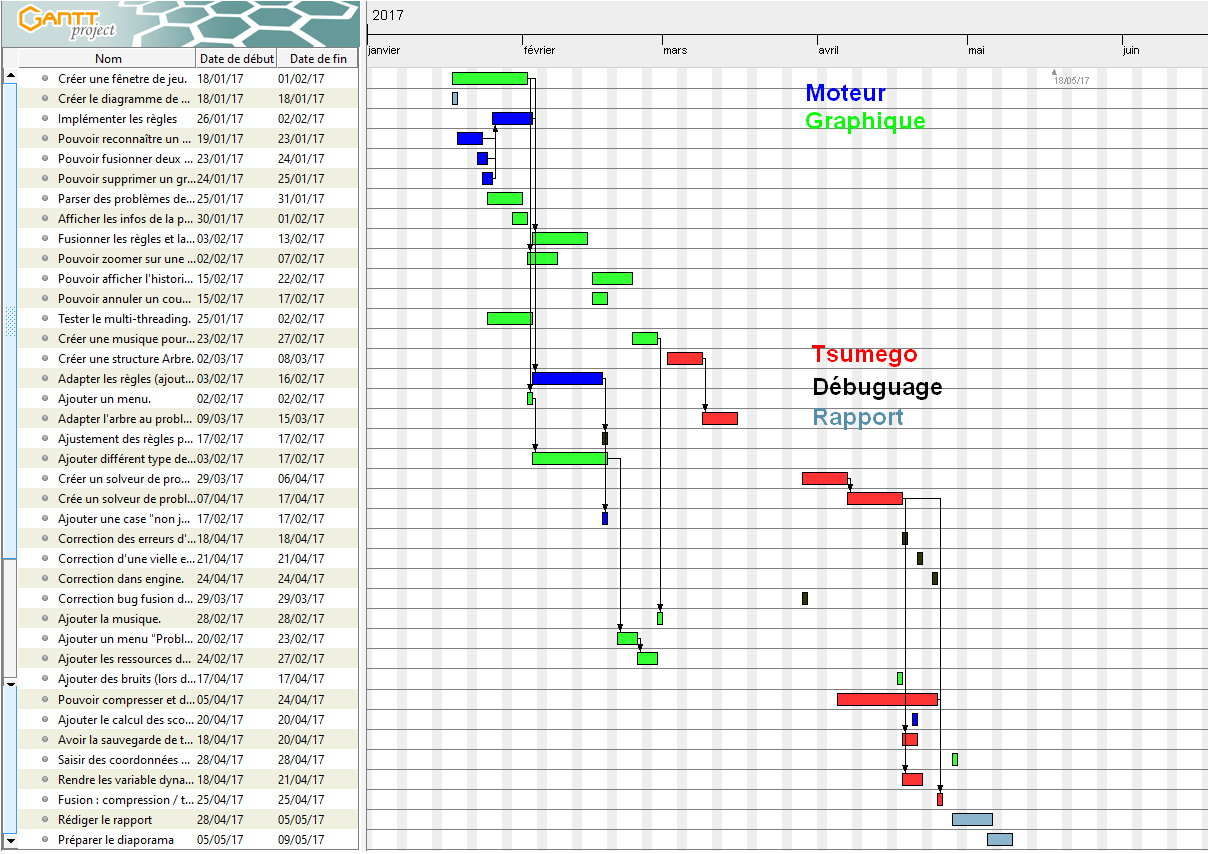
\includegraphics[scale=0.30]{figures/experiments/gantt-previ.png}
            \caption{Gantt Prévisionnel}
            \label{fig:gantt1}
            \end{figure} 
            
            \paragraph{}Évidemment dans un projet certaines parties prennent du retard et -plus rarement- de l'avance. Nous avons tout au long du projet tenu à jour notre planning pour le modifier en conséquence de notre avancement effectif.
            
        \subsubsection{Diagramme final}
            \begin{figure}[h!]
            \centering
            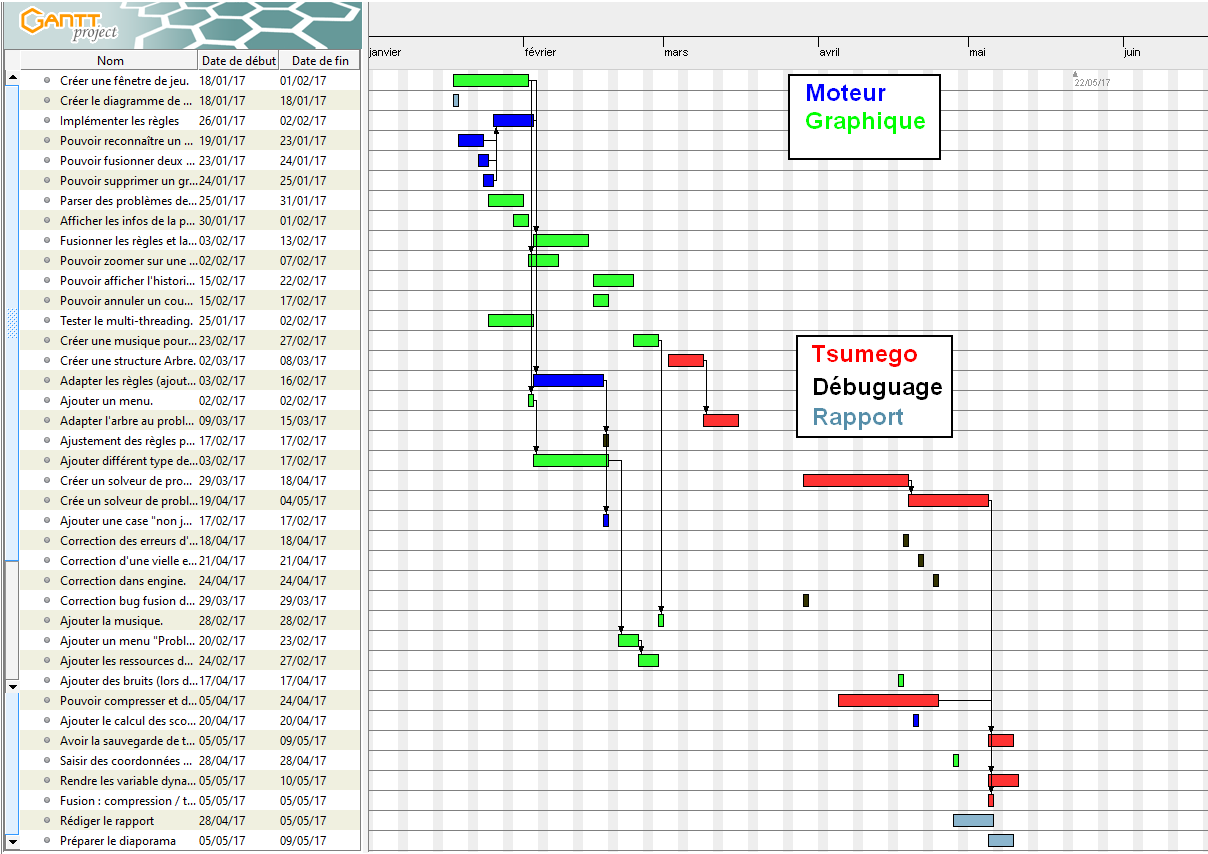
\includegraphics[scale=0.30]{figures/experiments/gantt-final.png}
            \caption{Gantt Final}
            \label{fig:gantt2}
            \end{figure}    
